
\documentclass{article}
\usepackage{graphicx}
\graphicspath{ {Assignment2Files/} }
\usepackage{color}

\usepackage{amsmath}
\usepackage{amssymb}
\usepackage{listings}
\usepackage{algorithm2e}
\usepackage{float}

\usepackage{hyperref}
\hypersetup{linktoc=all}

\usepackage{listings}
\usepackage{geometry}
\geometry{margin=1in}
\usepackage{color}
\definecolor{light-gray}{gray}{0.95}
\lstset{numbers=right, 
                numberstyle=\tiny, 
                breaklines=true,
                backgroundcolor=\color{light-gray},
                numbersep=5pt,
                xleftmargin=.5in,
                xrightmargin=.5in} 

\sloppy
\definecolor{lightgray}{gray}{0.5}
\setlength{\parindent}{0pt}

\begin{document}

\title{Lab 3: Simple Steganography}
\author{Brian Hosler \& Sarah Peachey }
\maketitle 

\abstract{Being able to hide information into images can be useful for
several reasons. If you want to determine if an image has been edited or
compressed, Least Significant Bit Hiding can be a technique for implementing
soft watermarking. But someone could easily remove the LSB plane, edit the
image, and then put the LSB plane back in. So more advanced algorithms like
Yeung-Mintzer Watermarking are used where a user must know the random seed
in order to extract the watermark. Therefore, it is more secure.}
\tableofcontents
\newpage


\section{Least Significant Bit Data Hiding}

Least significant bit hiding is when you take the MSB of the payload and
place it into the LSB of the host image. The below code executes a function that
examines one bit plane of an image, for every image. 

\begin{lstlisting}[language=Matlab]
pep=imread('Assingment 3 Files/peppers.tif');
bab=imread('Assingment 3 Files/baboon.tif');
figure
subplot(3,3,1)
imshow(pep)
for i=1:8
    subplot(3,3,10-i)
    imshow(getBP(pep,i))
end

figure
subplot(3,3,1)
imshow(bab)
for i=1:8
    subplot(3,3,10-i)
    imshow(getBP(bab,i))
end
\end{lstlisting}

The eight bit planes of the peppers.tif image and the baboon.tif image, are
shown below. As seen the MSB plane contains what appears to be a binary
version of the image, whereas the LSB plane contains what looks like noise.
All the bit planes in between transition from a recognizable image to noise.
The peppers.tif image becomes too noisy to recognize on bit plane 4,
whereas the baboon.tif has more high frequency content and becomes too
noisy on bit plane 5. The bit planes of the babbon.tif image are more noisy
because the high frequncy content means the bits change more often. 

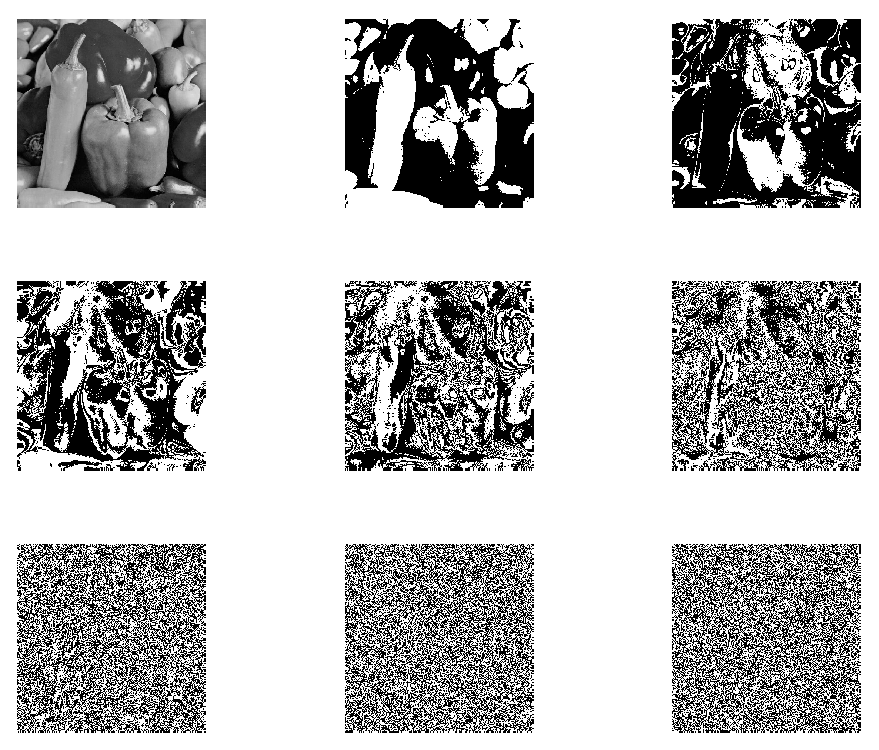
\includegraphics [width=4in]{lab3_01.eps}
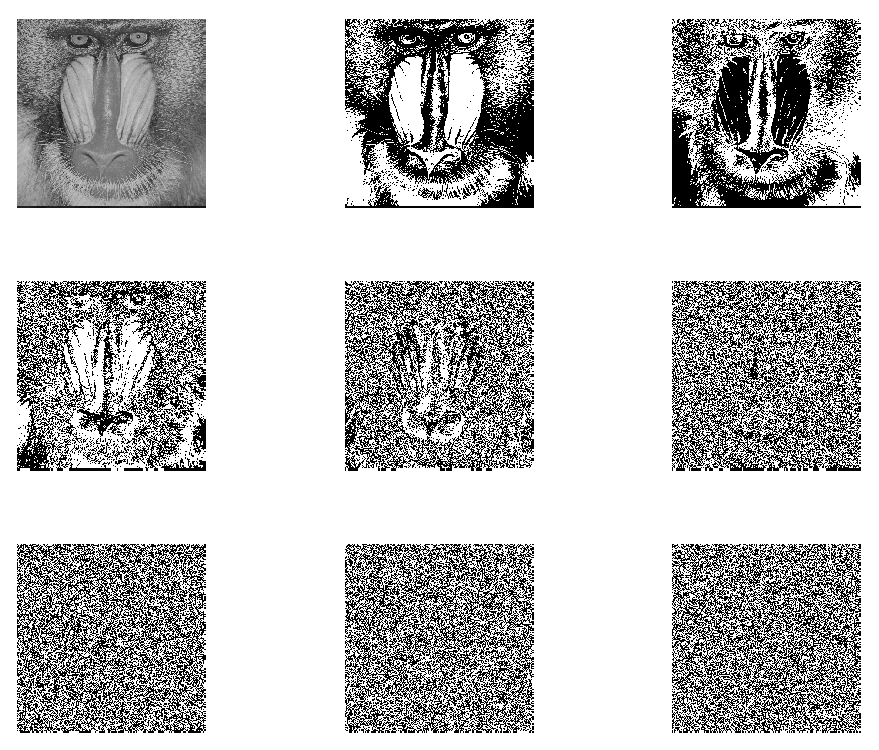
\includegraphics [width=4in]{lab3_02.eps}

The following code examines the different bit planes of several images to
see if there is any hidden content. As seen in the images, bit plane 2 was a
watermark in the first image, and bit plane 1 was a watermark in the last
two images. Then a function was written to replace the N least significant
bit planes from the one image with the N most significant bit planes from
another image. The top N layers of of Barabara.bmp are hidden in the
peppers.tif and baboon.tif images. The peppers image becomes distorted when
N=5, Barbara can be seen, and the peppers look choppy. 

\begin{lstlisting}
wmk1=imread('Assingment 3 Files/LSBwmk1.tiff');%2
wmk2=imread('Assingment 3 Files/LSBwmk2.tiff');%1
wmk3=imread('Assingment 3 Files/LSBwmk3.tiff');%1

figure
subplot(2,3,1); imshow(wmk1); title('Original')
subplot(2,3,4); imshow(getBP(wmk1,2)); title('Bit Plane 2')
subplot(2,3,2); imshow(wmk2); title('Original')
subplot(2,3,5); imshow(getBP(wmk2,1)); title('Bit Plane 1')
subplot(2,3,3); imshow(wmk3); title('Original')
subplot(2,3,6); imshow(getBP(wmk3,1)); title('Bit Plane 1')

barb=imread('Assingment 3 Files/Barbara.bmp');
figure
imshow(BPstitch(pep,barb,5))

type('getBP.m');
type('BPstitch.m');

\end{lstlisting}

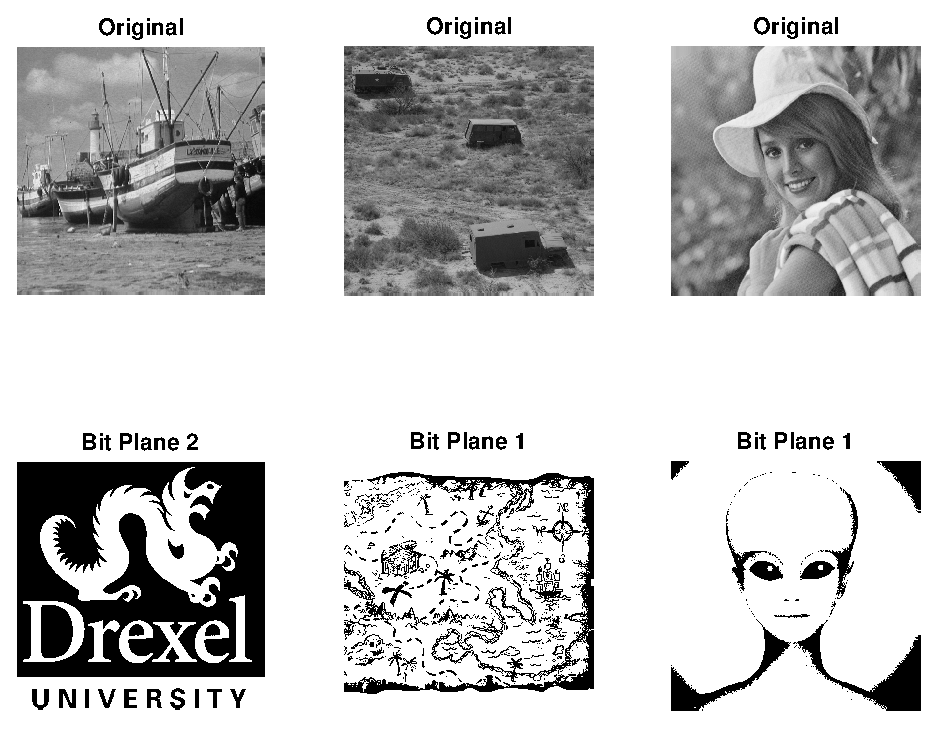
\includegraphics [width=4in]{lab3_03.eps}
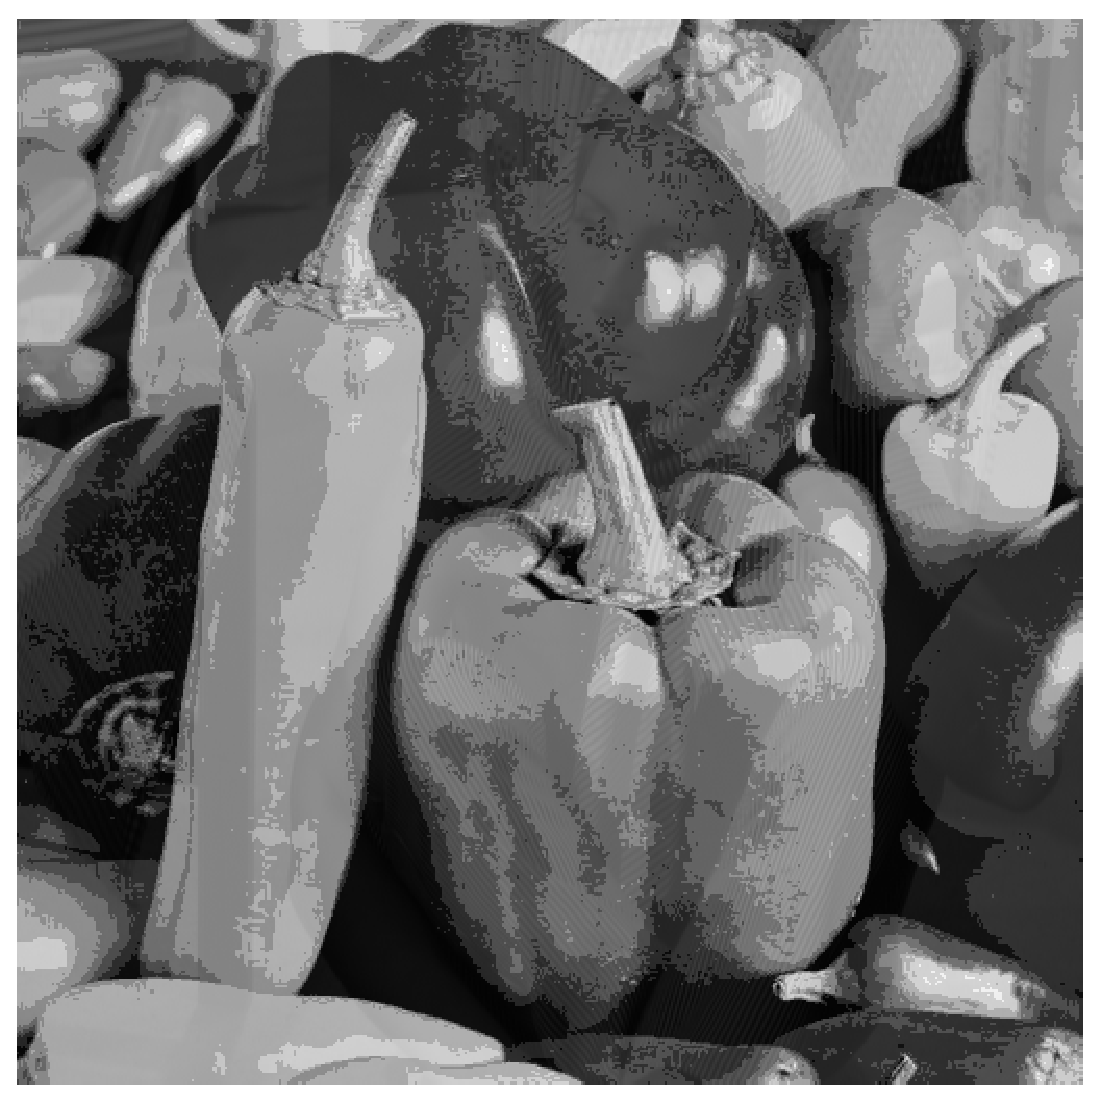
\includegraphics [width=4in]{lab3_04.eps}

This is the function used to get a bit plane from an image. 

\begin{lstlisting}[language=Matlab]
function [bp] = getBP(img,ind)
    bp=255*bitget(img,ind);

end
\end{lstlisting}

This is the function was used to replace the N least significant bits
of the host image with those of the payload image.

\begin{lstlisting}[language=Matlab]
function [encoded] = BPstitch(img,msg,N)
    encoded=uint8(zeros(size(img)));
    for i=(N+1):8
        encoded=encoded+(2^(i-1))*bitget(img,i);
    end
    if N==1
        encoded=encoded+bitget(msg,8);
    else
        for i=1:N
            encoded=encoded+(2^(N-i))*bitget(msg,9-i);
        end
    end

    encoded=uint8(encoded);
end
\end{lstlisting}



\section{Yeung-Mintzer Watermarking}
In this section, Yeung-Mintzer watermarking was implemented and tested
on several different images. The strengths and weaknesses compared to
LSB embedding were compared.

\begin{lstlisting}[language=Matlab]
key=256;
wmk=getBP(barb,8)>128;

img1=pep;
[marked1] = YMwatermark( img1,wmk,key );

img2=bab;
[marked2] = YMwatermark( img2,wmk,key );

% see the LSB of marked image
figure
imshow(getBP(marked1,1))
hold on
title('Yeung-Mintzer pepper - Bit plane 1')

figure
imshow(getBP(marked2,1))
hold on
title('Yeung-Mintzer baboon - Bit plane 1')

% get the PSNR
ym_psr_pep=psnr(pep, marked1)
ym_psr_bab=psnr(bab, marked2)

% LSB psnr
lsb_in_pep=BPstitch(pep,barb,1);
lsb_psnr_pep=psnr(pep, lsb_in_pep)

lsb_in_bab=BPstitch(bab,barb,1);
lsb_psnr_bab=psnr(bab, lsb_in_bab)

scrt=imread('Assingment 3 Files/YMwmkedKey435.tiff');
figure
imshow(YMcheck(scrt,435))


manbearpig1=mod(lsb_in_bab,16)+mod(pep,16)*16;
manbearpig2=mod(marked2,16)+mod(pep,16)*16;
figure
subplot(2,2,1)
imshow(manbearpig1)
subplot(2,2,2)
imshow(manbearpig2)
subplot(2,2,3)
imshow(getBP(manbearpig1,1))
subplot(2,2,4)
imshow(YMcheck(manbearpig2,256))
\end{lstlisting}

        \color{lightgray} \begin{verbatim}
ym_psr_pep =

   48.2109


ym_psr_bab =

   48.5526


lsb_psnr_pep =

   51.1422


lsb_psnr_bab =

   51.1391

\end{verbatim} \color{black}

YM watermarking resulted in a lower signal to noise ratio than the
LSB embedding. LSB embedding is guarenteed to change, at most, just
the least signifigant bit. YM watermarking however will result in
an indeterminate number of bit changes due to the random nature of
the lookup table. The signal to noise ratio of the LSB embedding was
consistently 3 dB higher than the YM embedding.
To verify the functionality of the Yueng-Mintzer decoder, an image was
decoded using the key 435, to reveal a tiled version of the Drexel
logo as the watermark.

    
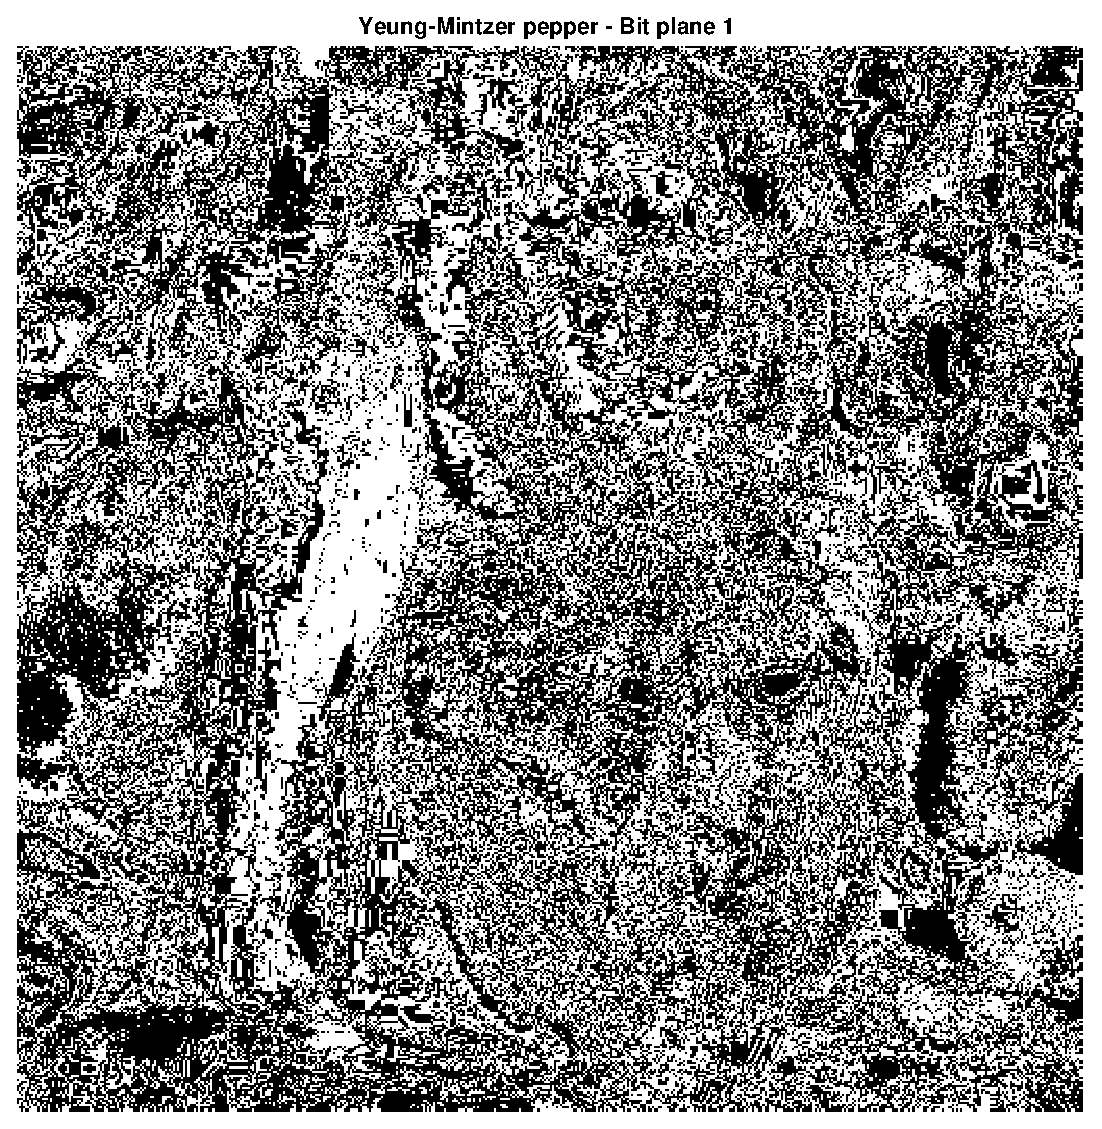
\includegraphics [width=4in]{lab3_05.eps}

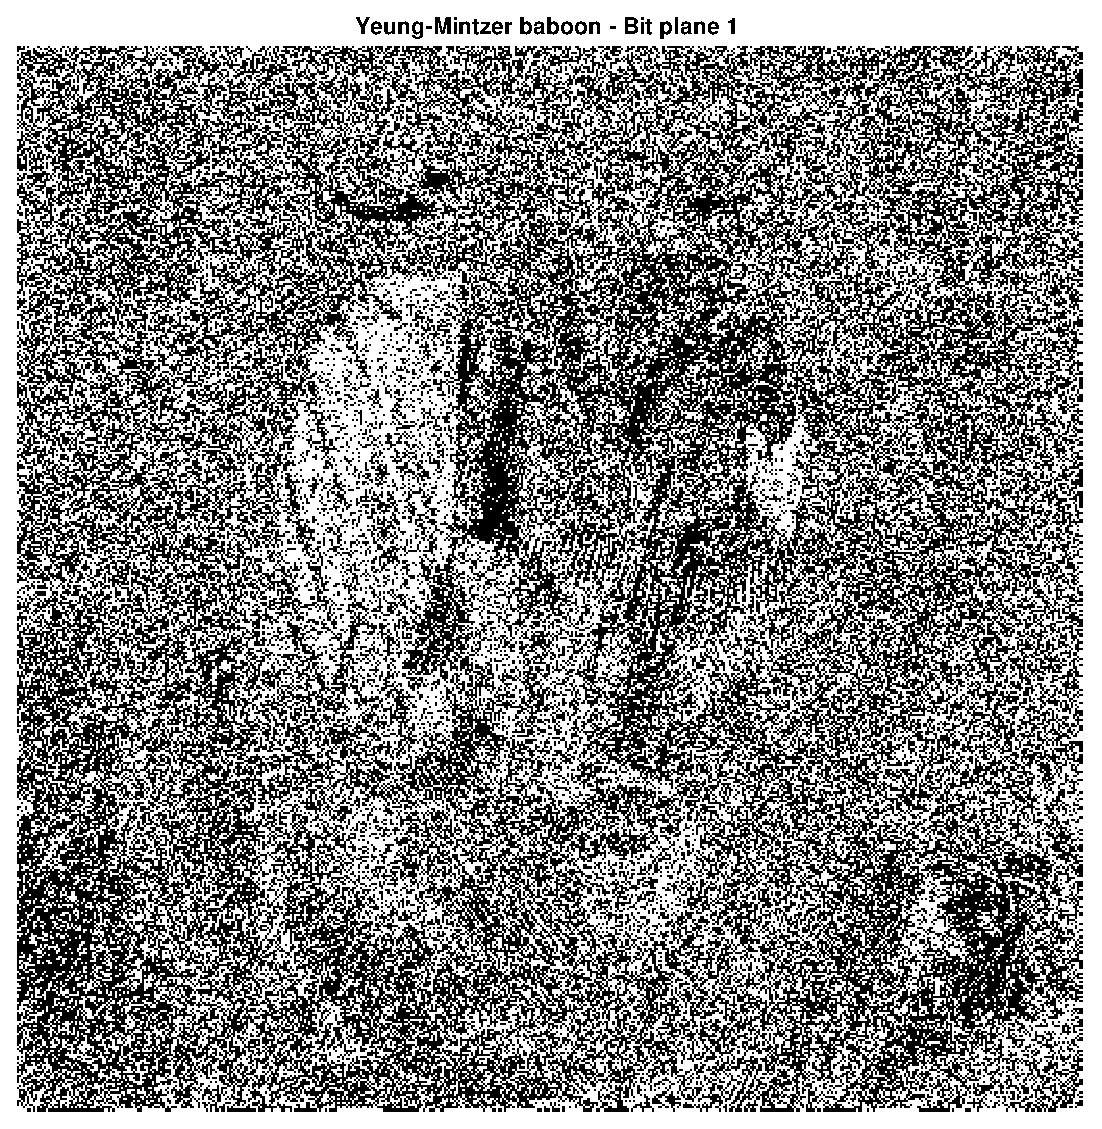
\includegraphics [width=4in]{lab3_06.eps}


\includegraphics [width=4in]{lab3_07.eps}

Next, LSB and YM watermarking were compared in terms of their fragility.
After detecting the watermark in the image with LSB watermarking, it is
easy to modify the image and replace the least significant bits with the
original watermark after. The YM watermark is harder to detect, and
unless the key to the lookup table is used, it is not possible to
recreate the watermark after editing the image.


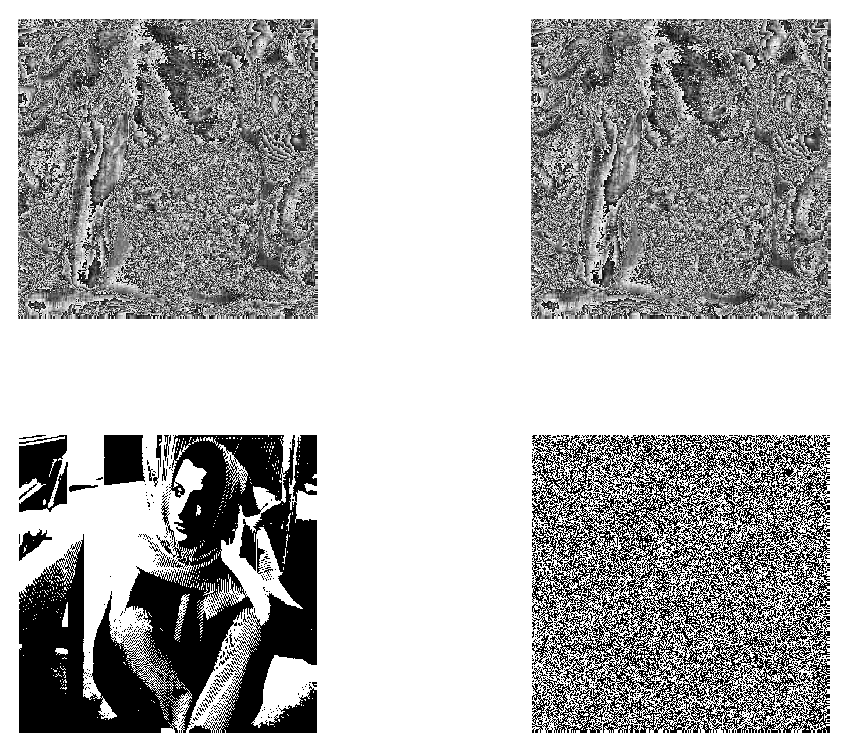
\includegraphics [width=4in]{lab3_08.eps}



\end{document}
    
